\documentclass[dvipdfmx]{jarticle}
\pagestyle{empty}
\usepackage{tikz}
\usetikzlibrary{calc,shapes}
\begin{document}
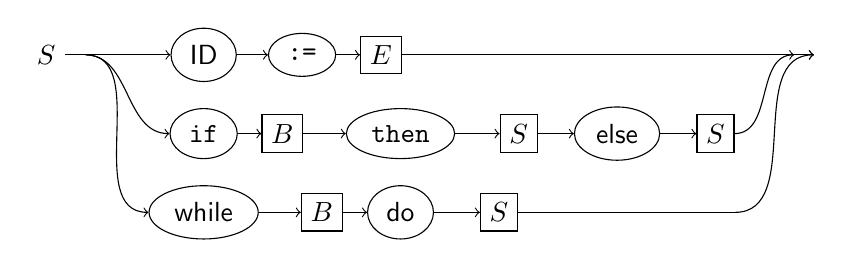
\begin{tikzpicture}
\coordinate (S0) at (0,0);
  \node (S-1) at ($(S0)+(-1,0)$) {$S$};
  \node[draw,ellipse] (S1) at ($(S0)+(1,0)$) {{\sf ID}};
  \node[draw,ellipse] (S11) at ($(S1)+(1.25,0)$) {\texttt{:=}};
  \node[draw] (S12) at ($(S11)+(1,0)$) {$E$};
  \node[draw,ellipse] (S2) at ($(S1)+(0,-1)$) {\texttt{if}};
  \node[draw] (S21) at ($(S2)+(1,0)$) {$B$};
  \node[draw,ellipse] (S22) at ($(S21)+(1.5,0)$) {\texttt{then}};
  \node[draw] (S23) at ($(S22)+(1.5,0)$) {$S$};
  \node[draw,ellipse] (S24) at ($(S23)+(1.25,0)$) {{\sf else}};
  \node[draw] (S25) at ($(S24)+(1.25,0)$) {$S$};
  \node[draw,ellipse] (S3) at ($(S0)+(1,-2)$) {{\sf while}};
  \node[draw] (S31) at ($(S3)+(1.5,0)$) {$B$};
  \node[draw,ellipse] (S32) at ($(S31)+(1,0)$) {{\sf do}};
  \node[draw] (S33) at ($(S32)+(1.25,0)$) {$S$};
  \path[->] (S-1) edge (S1) (S1) edge (S11) (S11) edge (S12) (S12) edge ($(S12)+(5.5,0)$);
  \path[->,out=0,in=180] ($(S0)+(-0.5,0)$) edge (S2);
  \path[->] (S2) edge (S21) (S21) edge (S22) (S22) edge (S23) (S23) edge (S24)
    (S24) edge (S25);
  \path[->,out=0,in=180] (S25) edge ($(S25)+(1,1)$);
  \path[->,out=0,in=180] ($(S0)+(-0.5,0)$) edge (S3);
  \path[->] (S3) edge (S31) (S31) edge (S32) (S32) edge (S33);
  \path[-] (S33) edge ($(S33)+(3,0)$);
  \path[->,out=0,in=180] ($(S33)+(3,0)$) edge ($(S33)+(4,2)$);
\end{tikzpicture}
\end{document}
